% !TEX root = ../../prj4projektdokumentation.tex
% SKAL STÅ I TOPPEN AF ALLE FILER FOR AT MASTER-filen KOMPILERES 

\section{Brugergrænseflade}
(Beskrivelse af skærm på PLC’en) \\
\subsection{Automatisk mode}
\begin{figure}[H] % (alternativt [H])
	\centering
	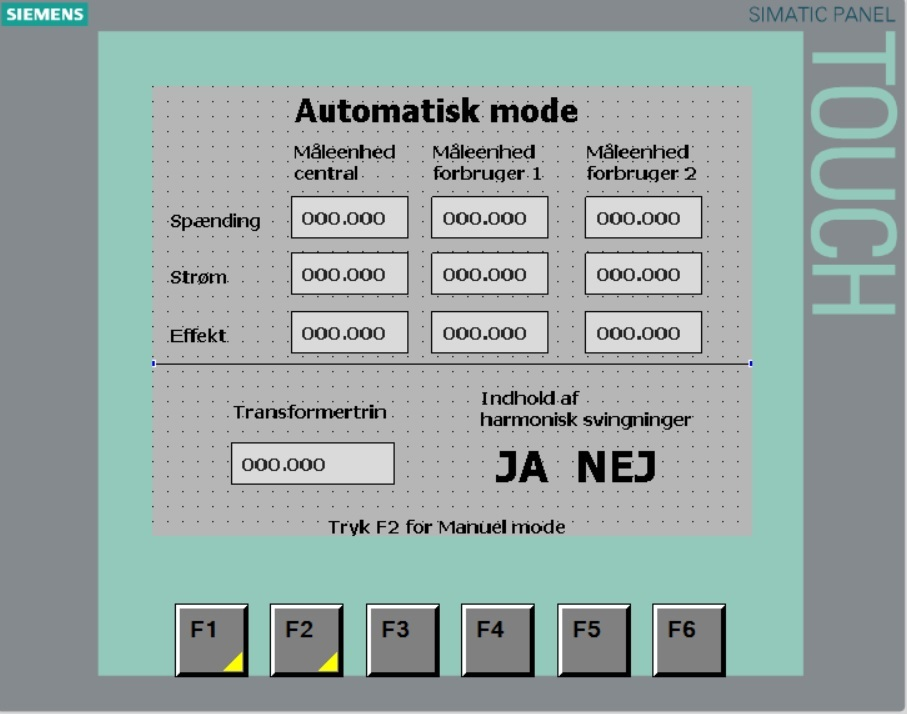
\includegraphics[width=0.9\textwidth]{Figure/HMIAutomatiskMode}
	\caption{HMI Automatisk mode}
	\label{fig:HMIAutomatikMode}
\end{figure}



\subsection{Manuel mode}
\begin{figure}[H] % (alternativt [H])
	\centering
	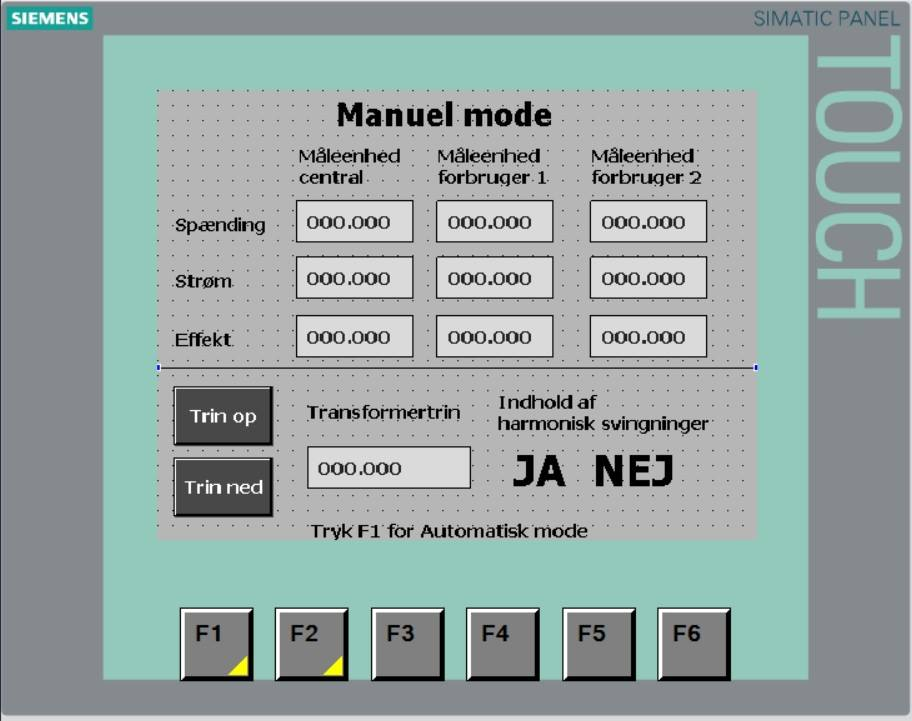
\includegraphics[width=0.9\textwidth]{Figure/HMIManuelMode}
	\caption{HMI Manuel mode}
	\label{fig:HMIManuelMode}
\end{figure}